
This method used to predict the reducible background allows to
have an inclusive measurement of the all the main reducible
backgrounds at the same time.

The control sample is obtained as a subset of the events that satisfy
the first step of the selection ({\it First Z} step, see
section~\ref{sec:zzcandsel}), requiring an additional pair of 
loose leptons of same sign (to avoid signal contamination) and same
flavour (SS-SF: $e^{\pm}e^{\pm}, \mu^{\pm}\mu^{\pm}$) .  The SS-SF
leptons are requested to pass the ${\rm SIP_{3D}}$ cut while no
identification or isolation requirements are imposed.  The
reconstructed invariant mass of the SS-SF leptons has to satisfy 
$m_{ \ell \ell} > 12$~GeV, $m_{ \ell \ell} < 120$~GeV,
the reconstructed four-lepton
invariant mass is required to satisfy $m_{4\ell} > 100~\GeVcc$,
and the QCD suppression cut (see~\ref{sec:zzcandsel}) is applied.
The inclusive number of reducible background events in the
signal region is derived from this set of events and from the probability for the
two additional leptons to pass the isolation and identification
analysis cuts, obtained from the fake rate measurement presented in section~\ref{sec:fakerate}.

Starting from the control sample previously described, the final
reducible background prediction in the signal region is given by the
following expression:
\begin{equation} 
\label{eq:FakeRateAA}
\begin{array}{cccc}
N^{\rm Z+X}_{\rm expect}  = & N^{\rm DATA}  \times   \rm{(\frac {OS}{SS})^{MC}}   \times &  
 f_1 \times f_2 
\end{array} 
\end{equation} 
where:
%
\begin{itemize}
\item $N^{\rm DATA}$ is the number of events in the control region,
\item $\rm{(\frac {OS}{SS})^{MC}}$ is a correction factor between opposite sign and same sign control samples,
\item $f_1$ and $f_2$ are the fake rates of each additional loose lepton, parameterised as a
   function of $p_T$ and $\eta$.
\end{itemize}

% ===========================================================================================================================================================
%  FAKE RATE DETERMINATION
% ===========================================================================================================================================================

\paragraph{Fake Rate Determination (SS Method)}
\label{sec:fakerate}

The lepton fake rates are determined in the very similar way as it was described before for the Opposite Sign method. Samples of $Z(\ell\ell)+e$ and $Z(\ell\ell)+\mu$ events are selected in the same way except that the mass window around the nominal Z mass is set to 40~GeV $< M_{inv}(\ell_{1},\ell_{2}) < $ 120~GeV, as in the signal region ("SS phase space").
Also, despite the cut on the missing transverse energy, a contamination of real leptons from WZ events is still visible at high $p_T$. This contribution is thus subtracted from the final fake rate, using the estimation given by the Monte Carlo. The fake rates for muon are shown in Fig.~\ref{fig:fakerates} for both muons in the barrel ($|\eta|<1.2$) and in the endcaps ($|\eta|>1.2$).

\begin{figure}[th]
\begin{center}
\subfigure [] {\resizebox{7.75cm}{!}{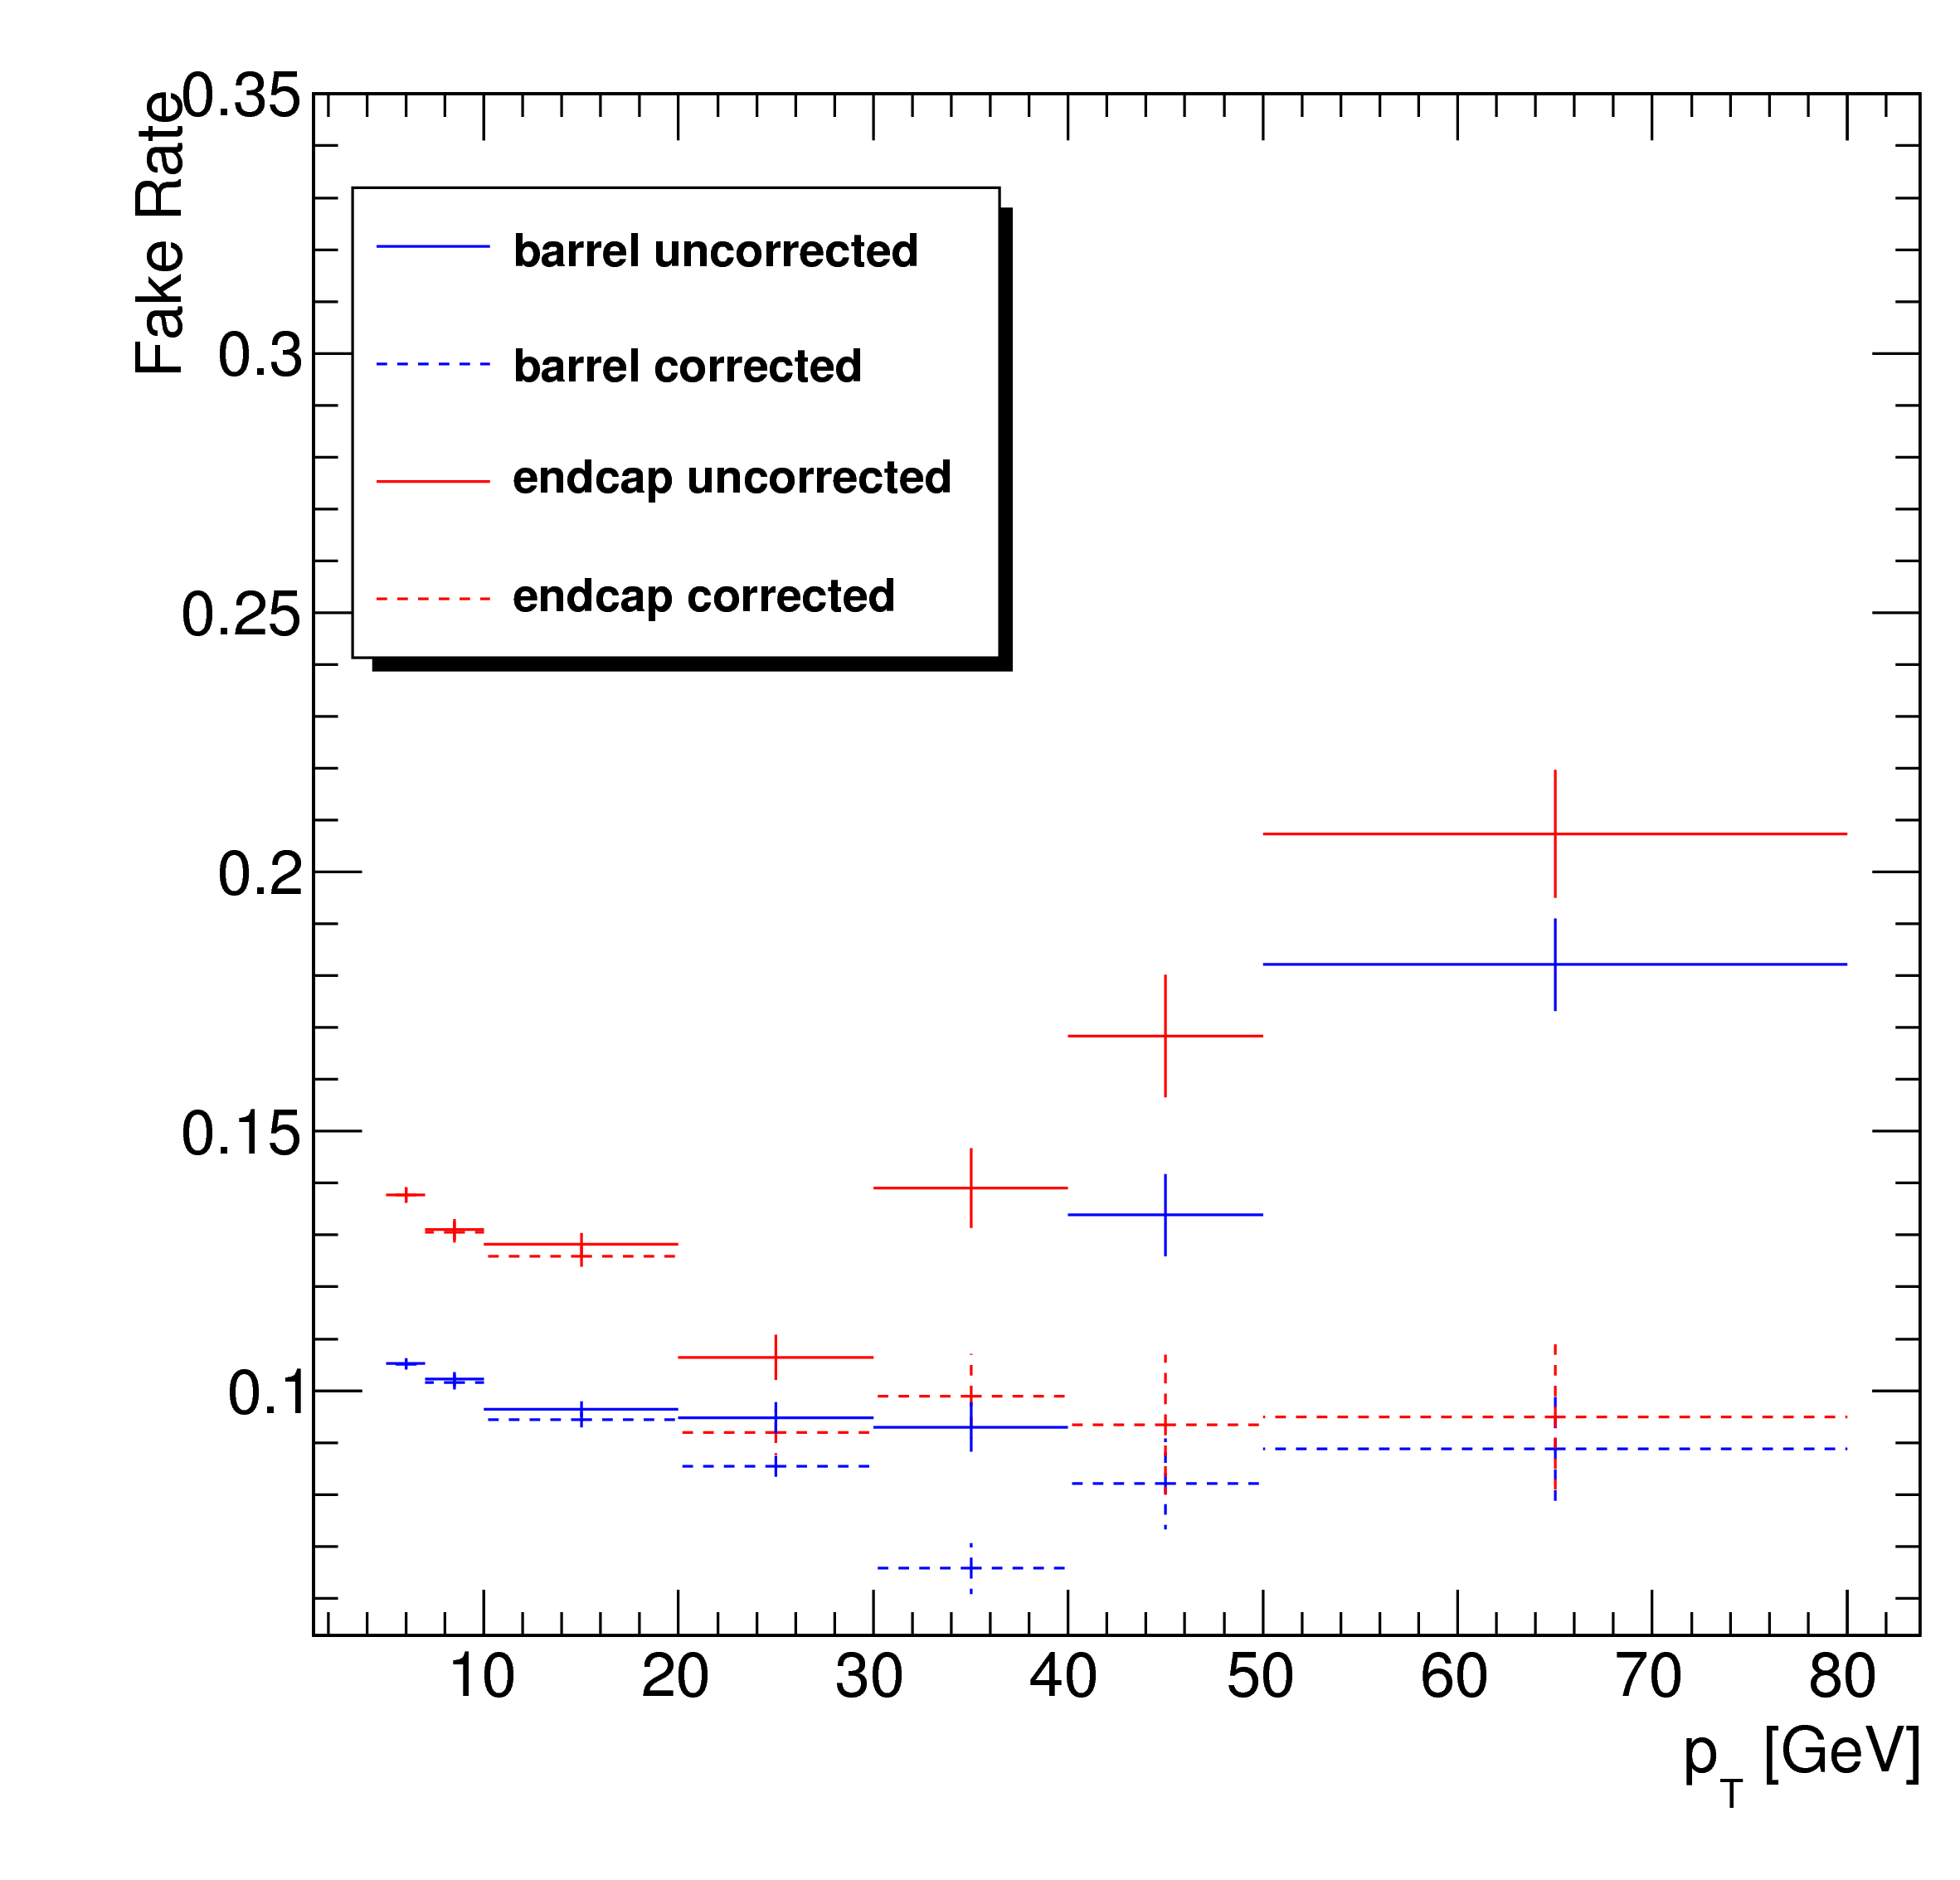
\includegraphics{Figures/RedBkg/FR_SS_muons.png}}}
\caption{
Fake rates as a function of the probe $p_T$ for muons which satisfy the loose selection criteria, measured in
a $Z(\ell\ell)+\ell$ sample in the $13$~TeV data.
The barrel selection includes electrons (muons) up to $|\eta|$ = 1.479 (1.2). The Fake rates are shown before (dotted lines) and after (plain line) the reoval of the WZ contribution from the simulation.
}
\label{fig:fakerates}
\end{center}\end{figure}

For electrons, events where a radiated photon makes an asymmetric conversion, where one low $p_T$ leg is not identified, contribute to the $Z + e$ sample that is used to measure the electron fake rate. While the requirement $|M_{inv}(\ell_{1},\ell_{2}) - M_{Z}| < 7 $~GeV ("OS phase space") largely suppresses FSR of photons radiated off the lepton legs, these radiations occur at a much larger rate in the "SS phase space". 
As a result of this enhanced
contribution from conversions, the electron fake rates measured
within the SR phase space  are larger than the "OS fake rates".

However, the relative fraction of FSR conversions is not the same in the "SS phase space"
and in the control sample (defined below) where the fake rates will be applied. A correction
accounting for this difference must be applied to the fake rates measured within 
the SS phase space, in order to obtain
average fake rates that are appropriate for the control sample.
To determine this correction,
several fake rate samples of $Z(ll) + e$ events are defined by applying different 
cuts on $M_{inv}(\ell_{1},\ell_{2})$ or on $M_{inv}(\ell_{1},\ell_{2}, e)$.
In addition to the "OS fake rate sample", where $|M_{inv}(\ell_{1},\ell_{2}) - M_{Z}| < 7 $~GeV ensures
a minimal amount of conversions from FSR photons, one defines a sample that is
maximally enriched in FSR conversions by
$ | M_{inv}(\ell_{1},\ell_{2}, e) - M_Z | < $~5~GeV,
as well as samples with 
an intermediate contamination from FSR conversions (60~GeV $< M_{inv}(\ell_{1},\ell_{2}) < $ 120~GeV).
In each sample, one determines, in several $(p_T, \eta)$ bins for the loose electron:
\begin{itemize}
 \item the fake rate ratio;
 \item the average value of the expected inner missing hits ($N_{miss. hits}$ in the following), variable useful to tag conversions. 
\end{itemize}
%

%\begin{figure}[th]
%\begin{center}
%    \subfigure [] {\resizebox{7.75cm}{!}{\includegraphics{Figures/RedBkg/COMP_VECturnon_TG_Lep3_pT_all_EB_afterMET_LHCP414_SS.pdf}}} 
%    \subfigure [] {\resizebox{7.75cm}{!}{\includegraphics{Figures/RedBkg/COMP_VECturnon_TG_Lep3_pT_all_EE_afterMET_LHCP414_SS.pdf}}} \\
%\caption{
%Fake rates measured for various phase spaces: 40~GeV $< M_{inv}(\ell_{1},\ell_{2}) < $ 120~GeV, $|M_{inv}(\ell_{1},\ell_{2}) - M_{Z}| < $ 7 GeV (blue), 60~GeV $< M_{inv}(\ell_{1},\ell_{2}) < $ 120~GeV (red), $ | M_{inv}(\ell_{1},\ell_{2}, e) - M_Z | < $~5~GeV (green), for electrons in the barrel (left) and in the endcaps (right).
%Results are produced at 13~TeV with 36.8~fb$^{-1}$ data.
%}
%\label{fig:FRSSvarious}
%\end{center}
%\end{figure}

In a given $(p_T, \eta)$  bin, both the measured fake rate and the
average $ < N_{miss. hits} > $ are expected to grow linearly with the fraction
of conversions. 
Hence, one expects a linear dependence of the fake rate with respect to $ < N_{miss. hits} > $.
This linear behaviour is demonstrated in Fig.~\ref{fig:FRvsNHits}, and linear fits are made
in each $(p_T, \eta)$  bin, which relate the fake rate to $ < N_{miss. hits} > $.

\begin{figure}[th]
\begin{center}
    \subfigure [] {\resizebox{7.75cm}{!}{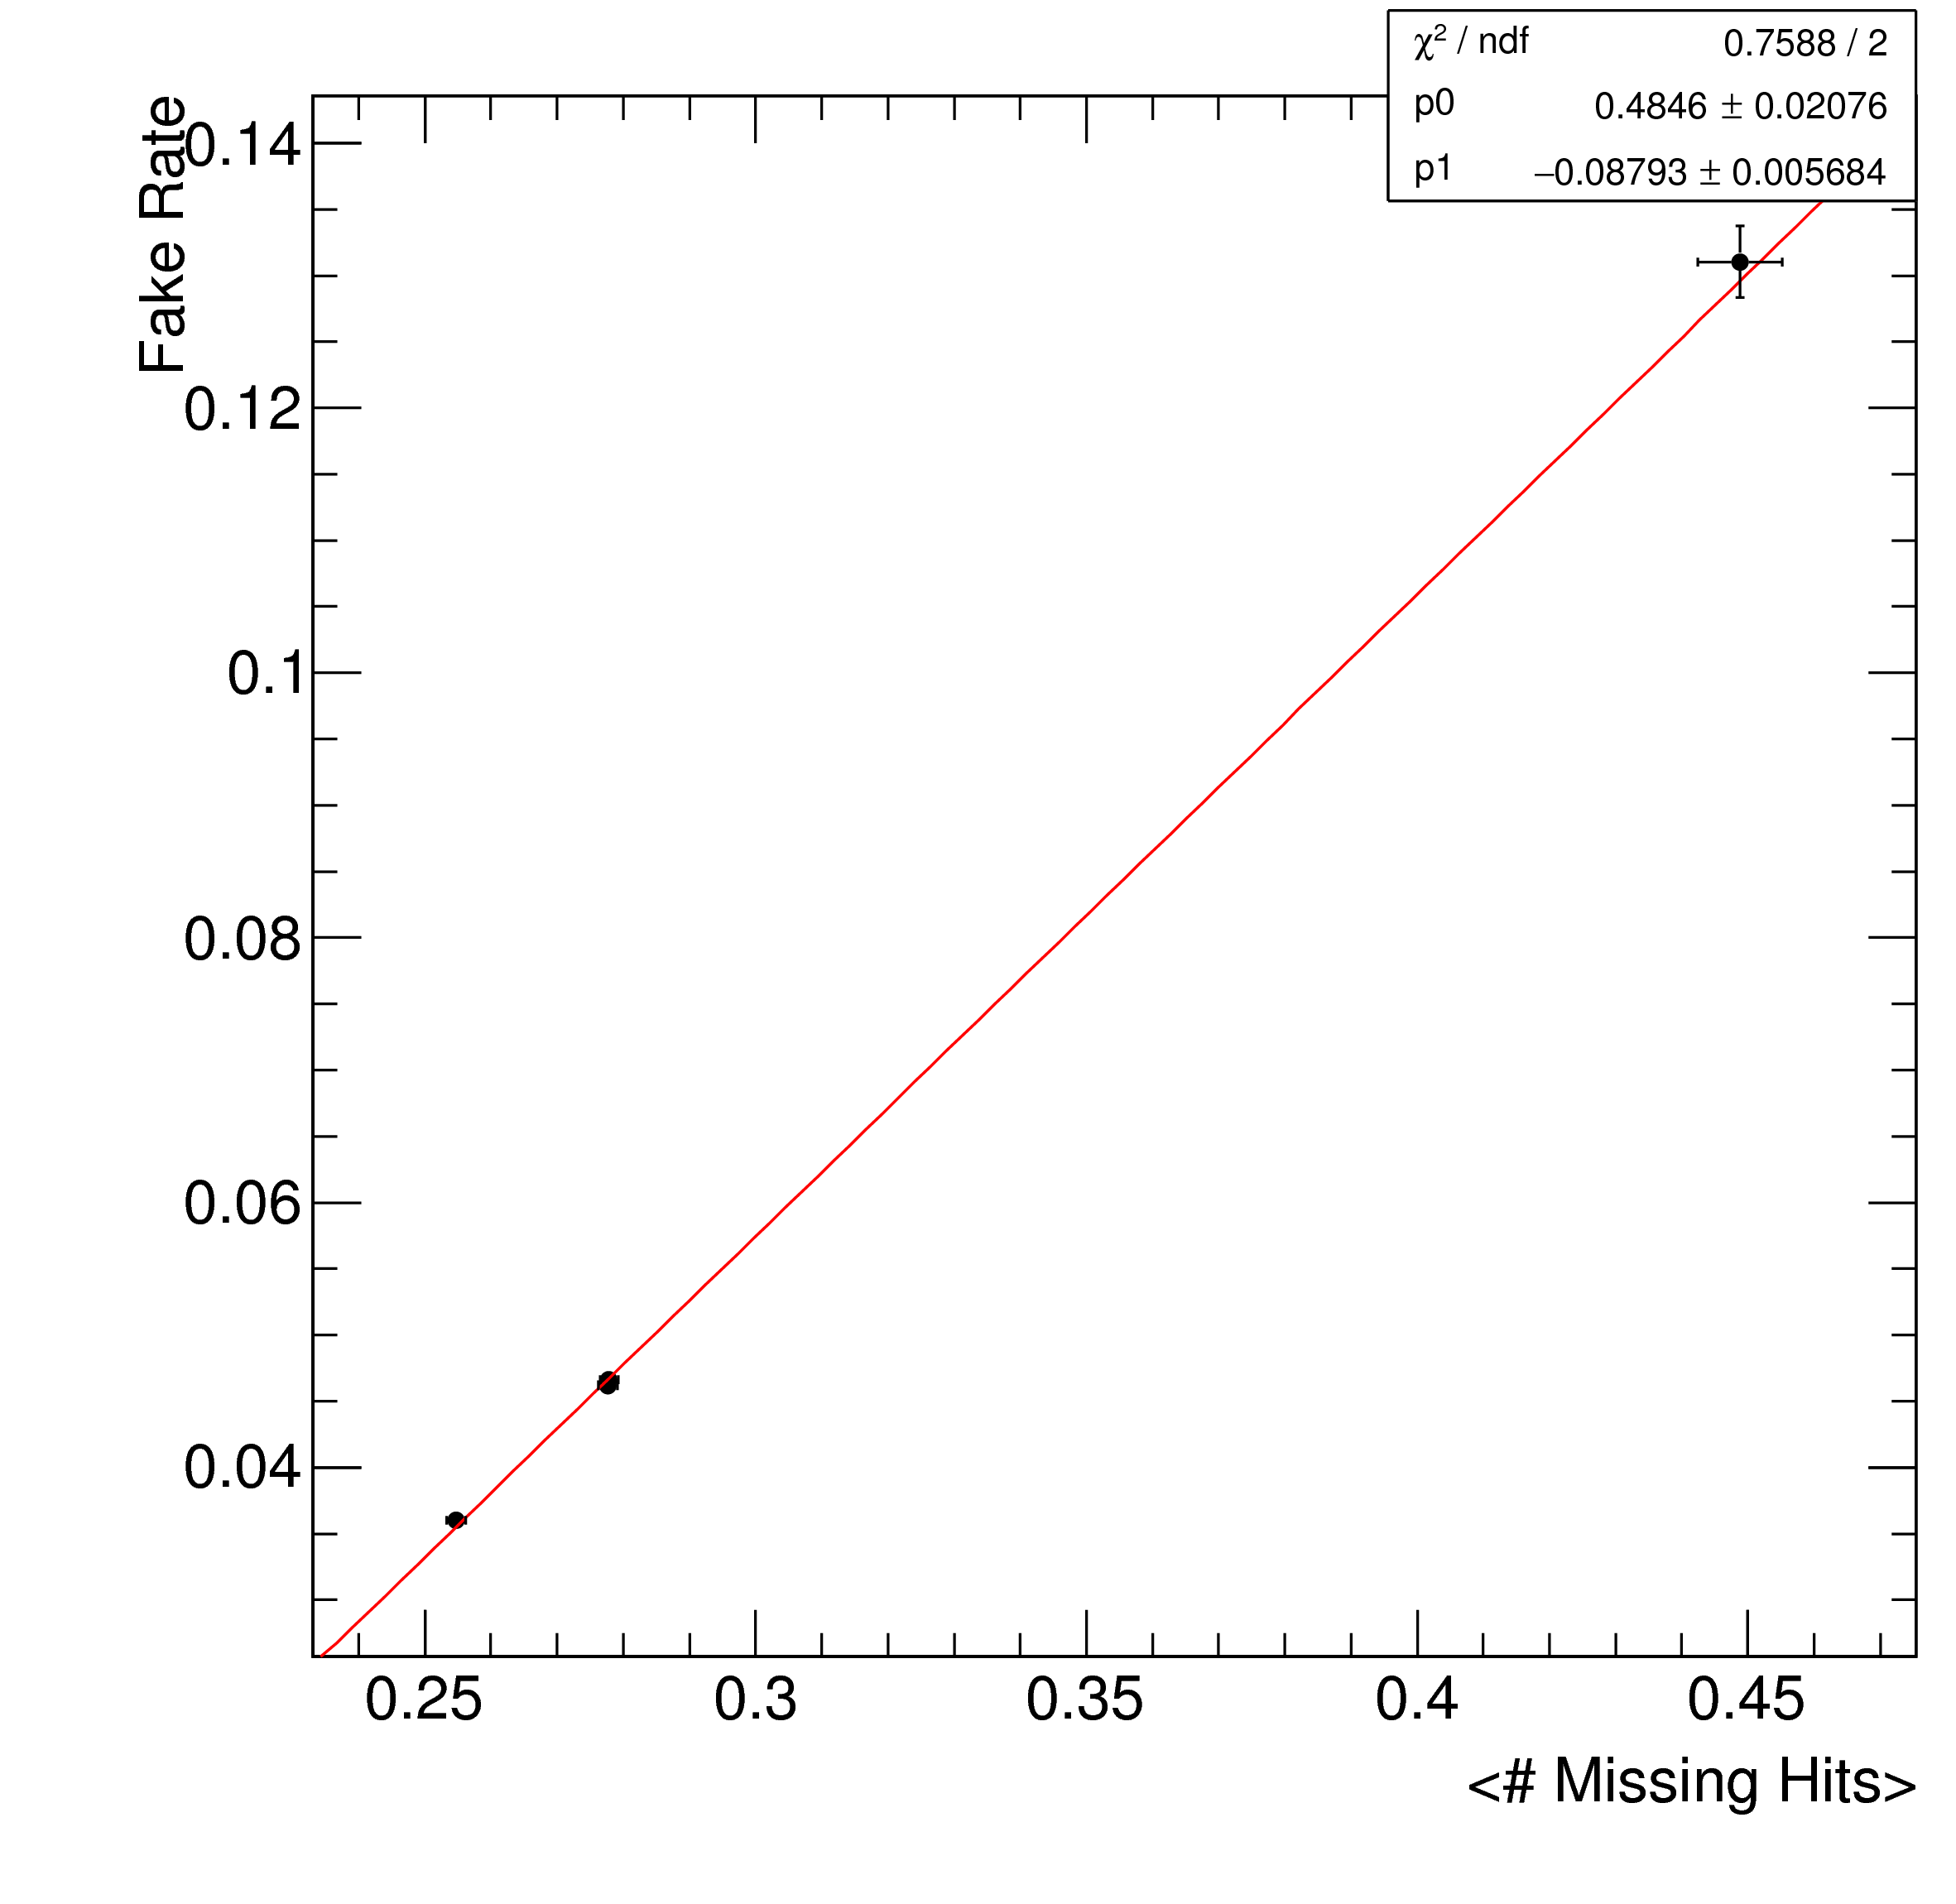
\includegraphics{Figures/RedBkg/FR_MissingHits_graph_eta_0_pT_0.png}}} 
    \subfigure [] {\resizebox{7.75cm}{!}{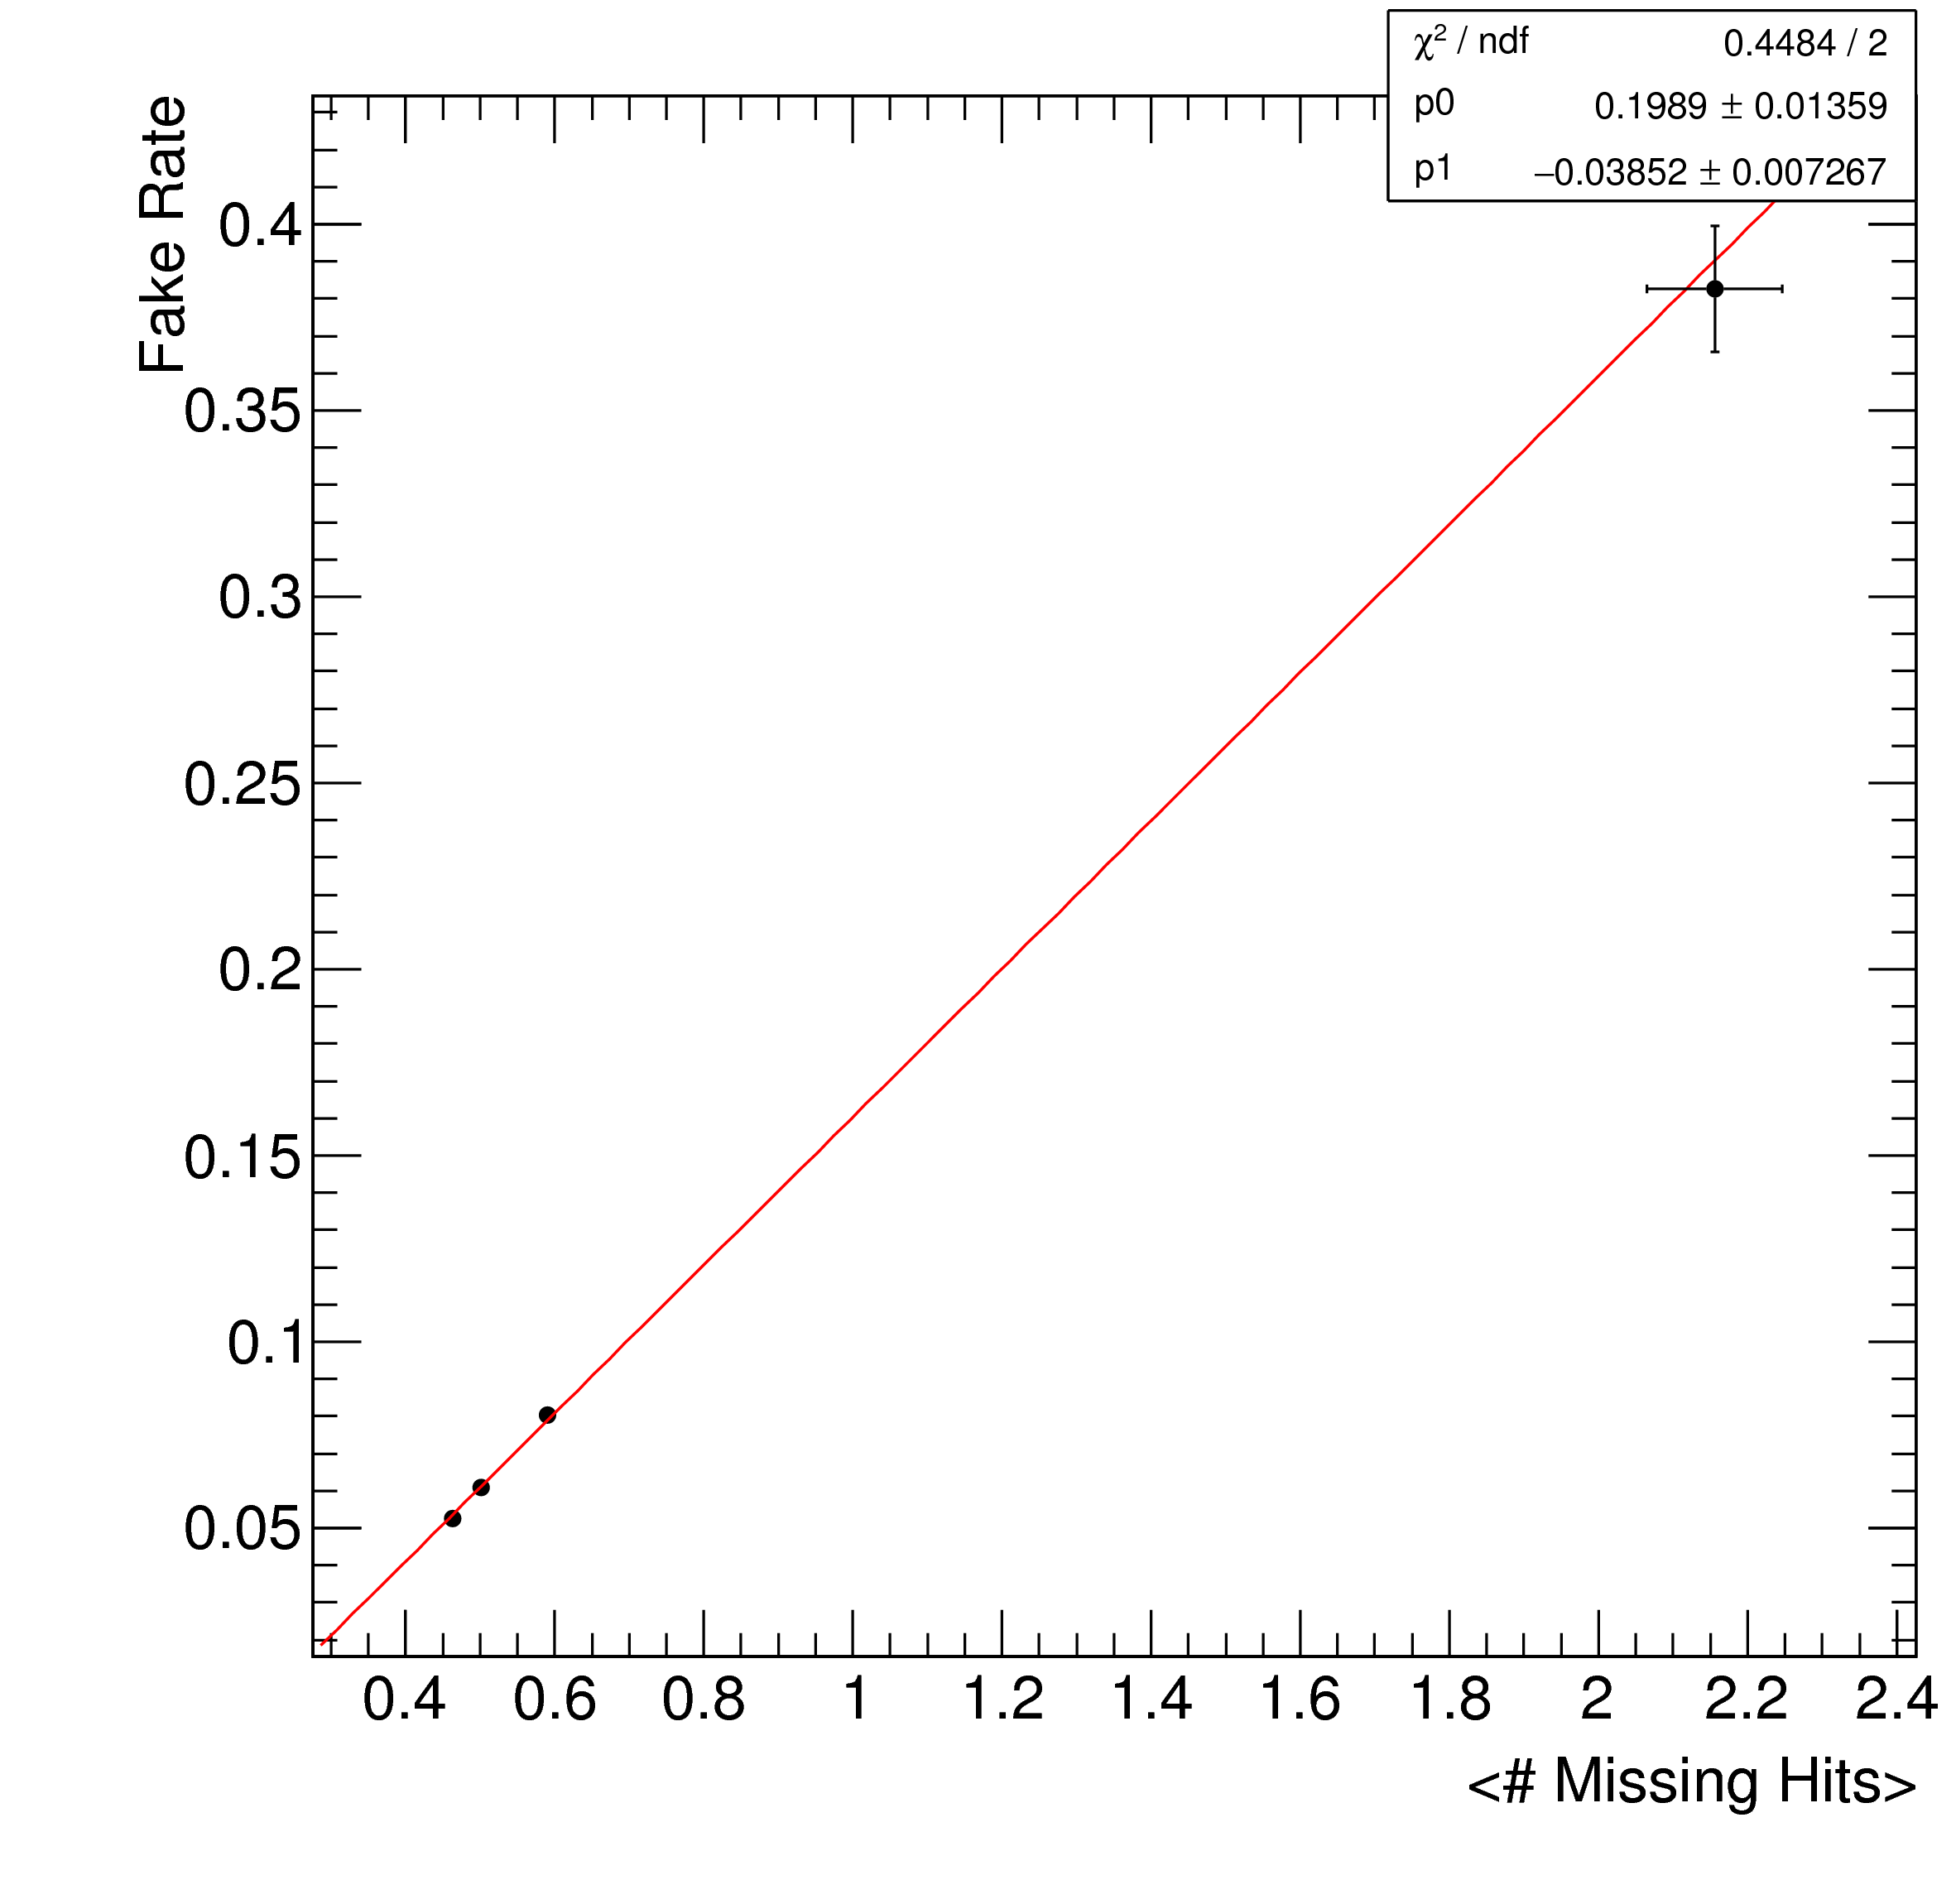
\includegraphics{Figures/RedBkg/FR_MissingHits_graph_eta_1_pT_3.png}}} 
\caption{
Examples of the correlation between the fake rate and the fraction of loose electrons 
for which the track has one missing hit in the pixel detector for  $7<p_T<10$~GeV electrons in the barrel (left) and for $20<p_T<30$~GeV electrons in the endcaps (right).
Each dot shows the measurements made in a given $Z$ + loose $e$ sample.
Results are produced at 13~TeV with 36.8~fb$^{-1}$ data.
}
\label{fig:FRvsNHits}
\end{center}
\end{figure}

Finally, one looks at the loose electrons in the control sample where the fake rate will be applied, and one measures, in each
$(p_T, \eta)$ bin, $<N_{miss. hits}>$.
The proper average fake rate corresponding to the control sample is then determined from the
linear relation derived previously.
Figure~\ref{fig:FRAAcorrected} shows examples of the resulting corrected fake rates, together with the
fake rates measured in the SS phase space. % and the A fake rates.
It can be seen that the correction for the actual fraction of conversions that is present in the
control sample lowers the fake rates considerably with respect to what is measured
in the SS phase space.
The determination of these corrected fake rates mostly suffers from the limited statistics of the
control sample, which translates into a large uncertainty on $<N_{miss. hits}>$, the error on each dot being the fake rate obtained from the linear relations using the error on the $<N_{miss. hits}>$.

\begin{figure}[th]
\begin{center}
    \subfigure [] {\resizebox{7.75cm}{!}{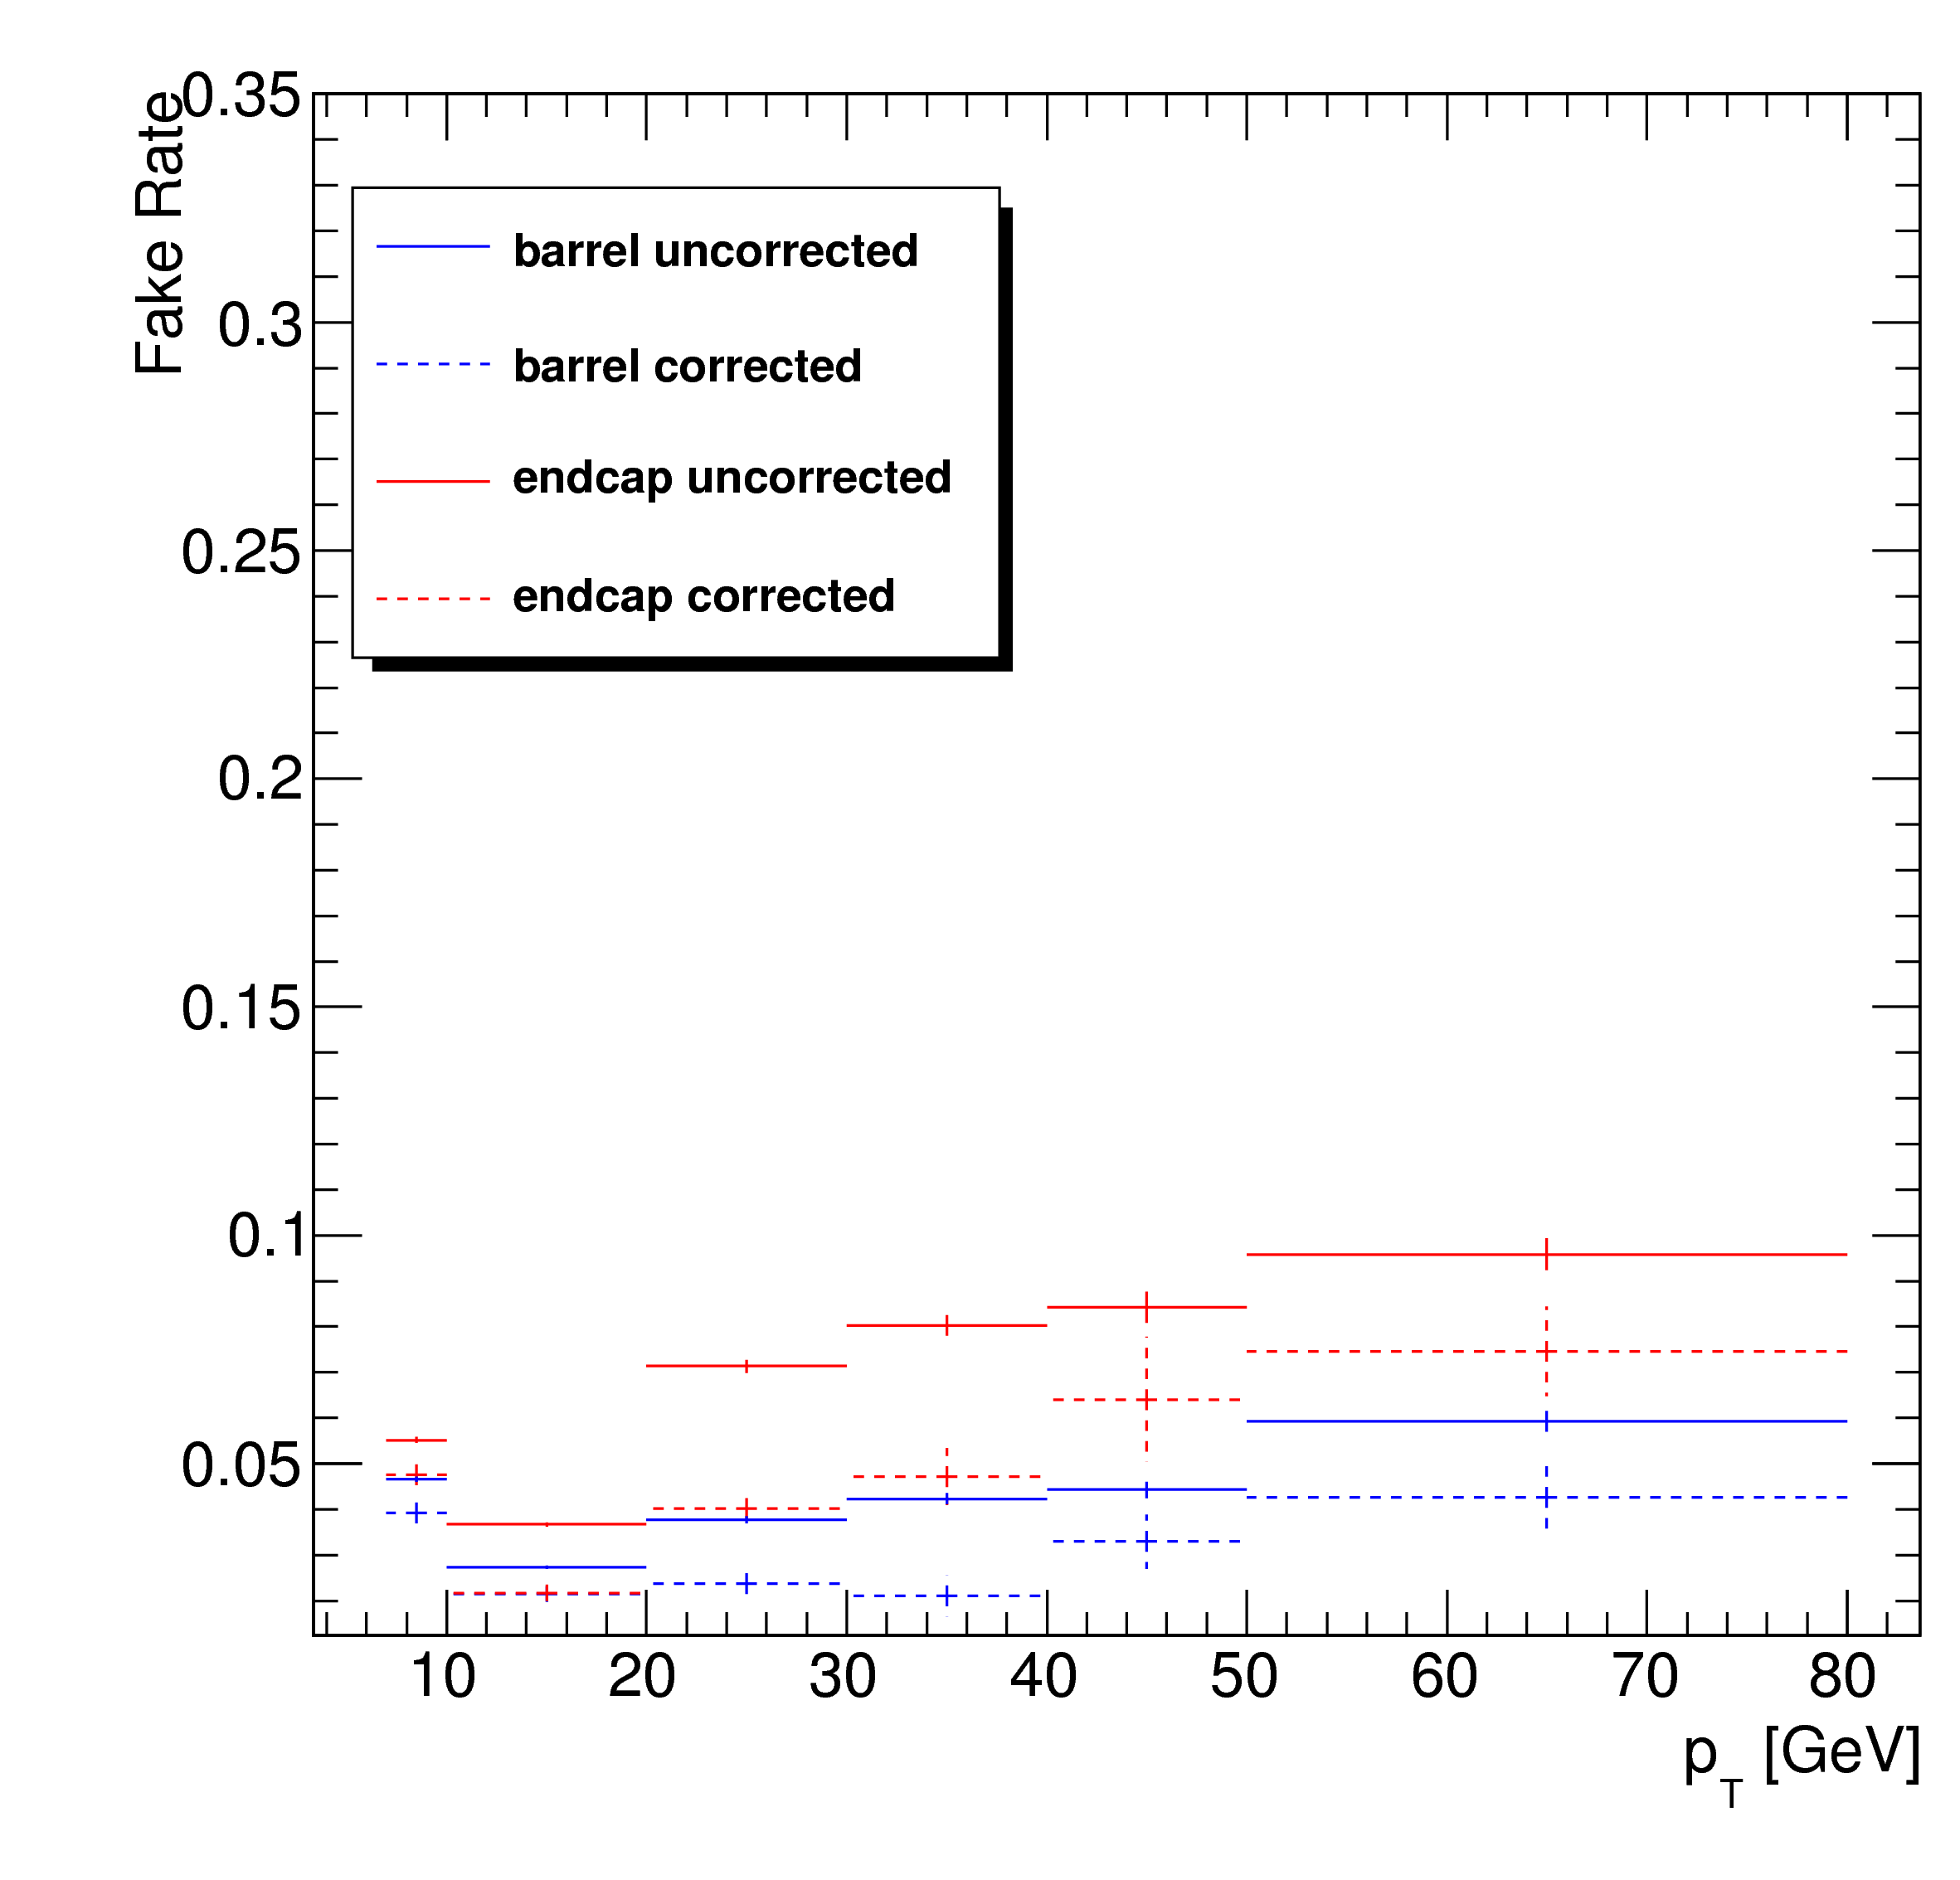
\includegraphics{Figures/RedBkg/FR_SS_electrons.png}}}
\caption{Average fake rates to be applied to the control sample of SS Method (plain line), compared to
  the fake rates measured in the SS phase space (dotted line), for electrons in the barrel (blue) and in the endcaps (red).
  Results are produced at 13~TeV with 2018 data.
  } % and in the A fake rate sample (open squares).
\label{fig:FRAAcorrected}
\end{center}
\end{figure}

% ===========================================================================================================================================================
%  FAKE RATE APPLICATION
% ===========================================================================================================================================================

%\subsubsection{Fake Rate Application}
\paragraph{Fake Rate Application (SS Method)}
%Figures~\ref{fig:ZjetControlRegionShapes}
Figure~\ref{fig:ZjetControlRegionShapes13TeV} shows the invariant mass
distribution of events in control samples with SS-SF loose leptons,
for channels with loose electrons ($4e$ and $2\mu2e$) and channels
with loose muons ($4\mu$ and $2e2\mu$), for the $13$~TeV dataset. 
The prediction from the Monte-Carlo simulation is also shown.

A good agreement is achieved between data and MC for the channels
with loose electrons. The agreement is not as good for loose muons
but this has no impact on the final result as only data are used in the end.  

The differences in rates between OS and SS samples are used to
 compute the correction factor in~equation~\ref{eq:FakeRateAA} for the
 final data-driven estimation. They are given in table~\ref{tab:OSSS}.

\begin{table}[h]
% \scriptsize
\begin{center}
    \begin{tabular}{ | l | c | c | c |  c | }  \hline
   channel  &  4e  &  2$\mu$ 2e   &  4 $\mu$   &   2e 2$\mu$   \\ \hline
   
   OS/SS    &  1.00 $\pm$ 0.01  &  1.00 $\pm$ 0.01   &  1.03 $\pm$ 0.02  &  1.03 $\pm$ 0.03 \\ \hline
        \end{tabular} 
    \caption{ The OS / SS ratios used in the Same-Sign Method. }
    \label{tab:OSSS}
\end{center}
\end{table}


\begin{figure}[!htb]
\begin{center}
\subfigure[]{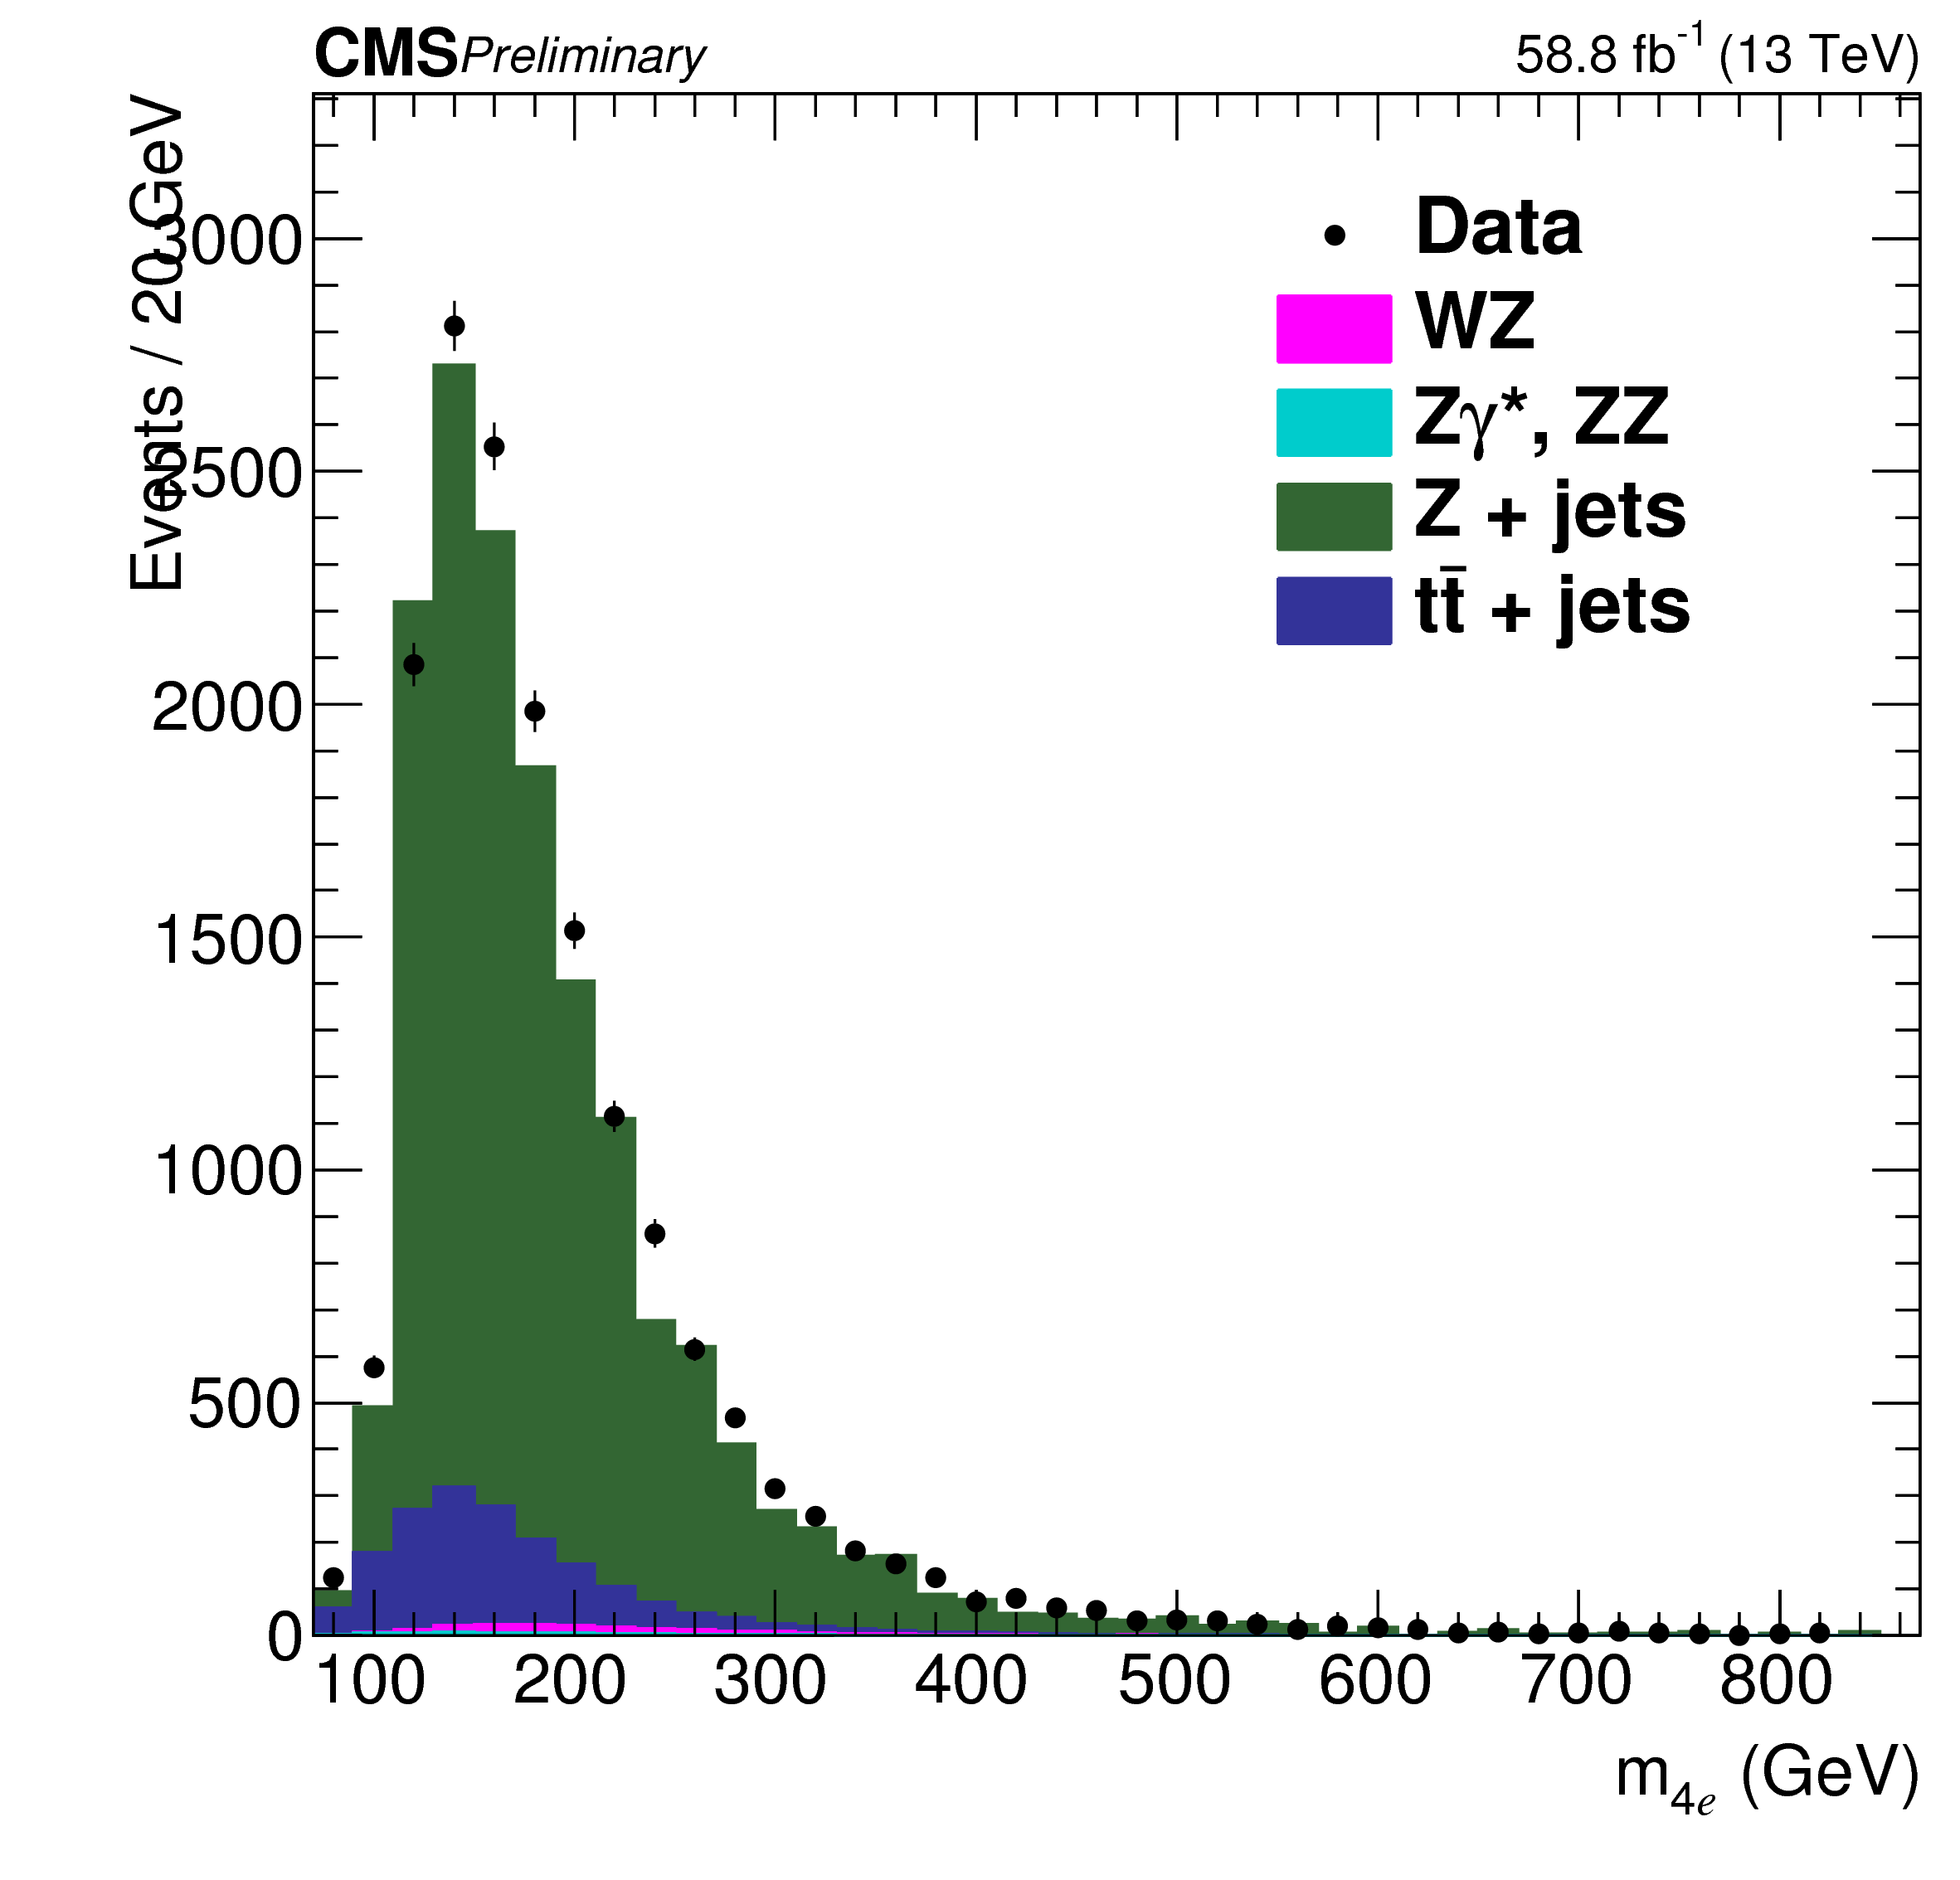
\includegraphics[width=0.45\textwidth]{Figures/RedBkg/M4l_SS_4e_Inclusive.png}} 
\subfigure[]{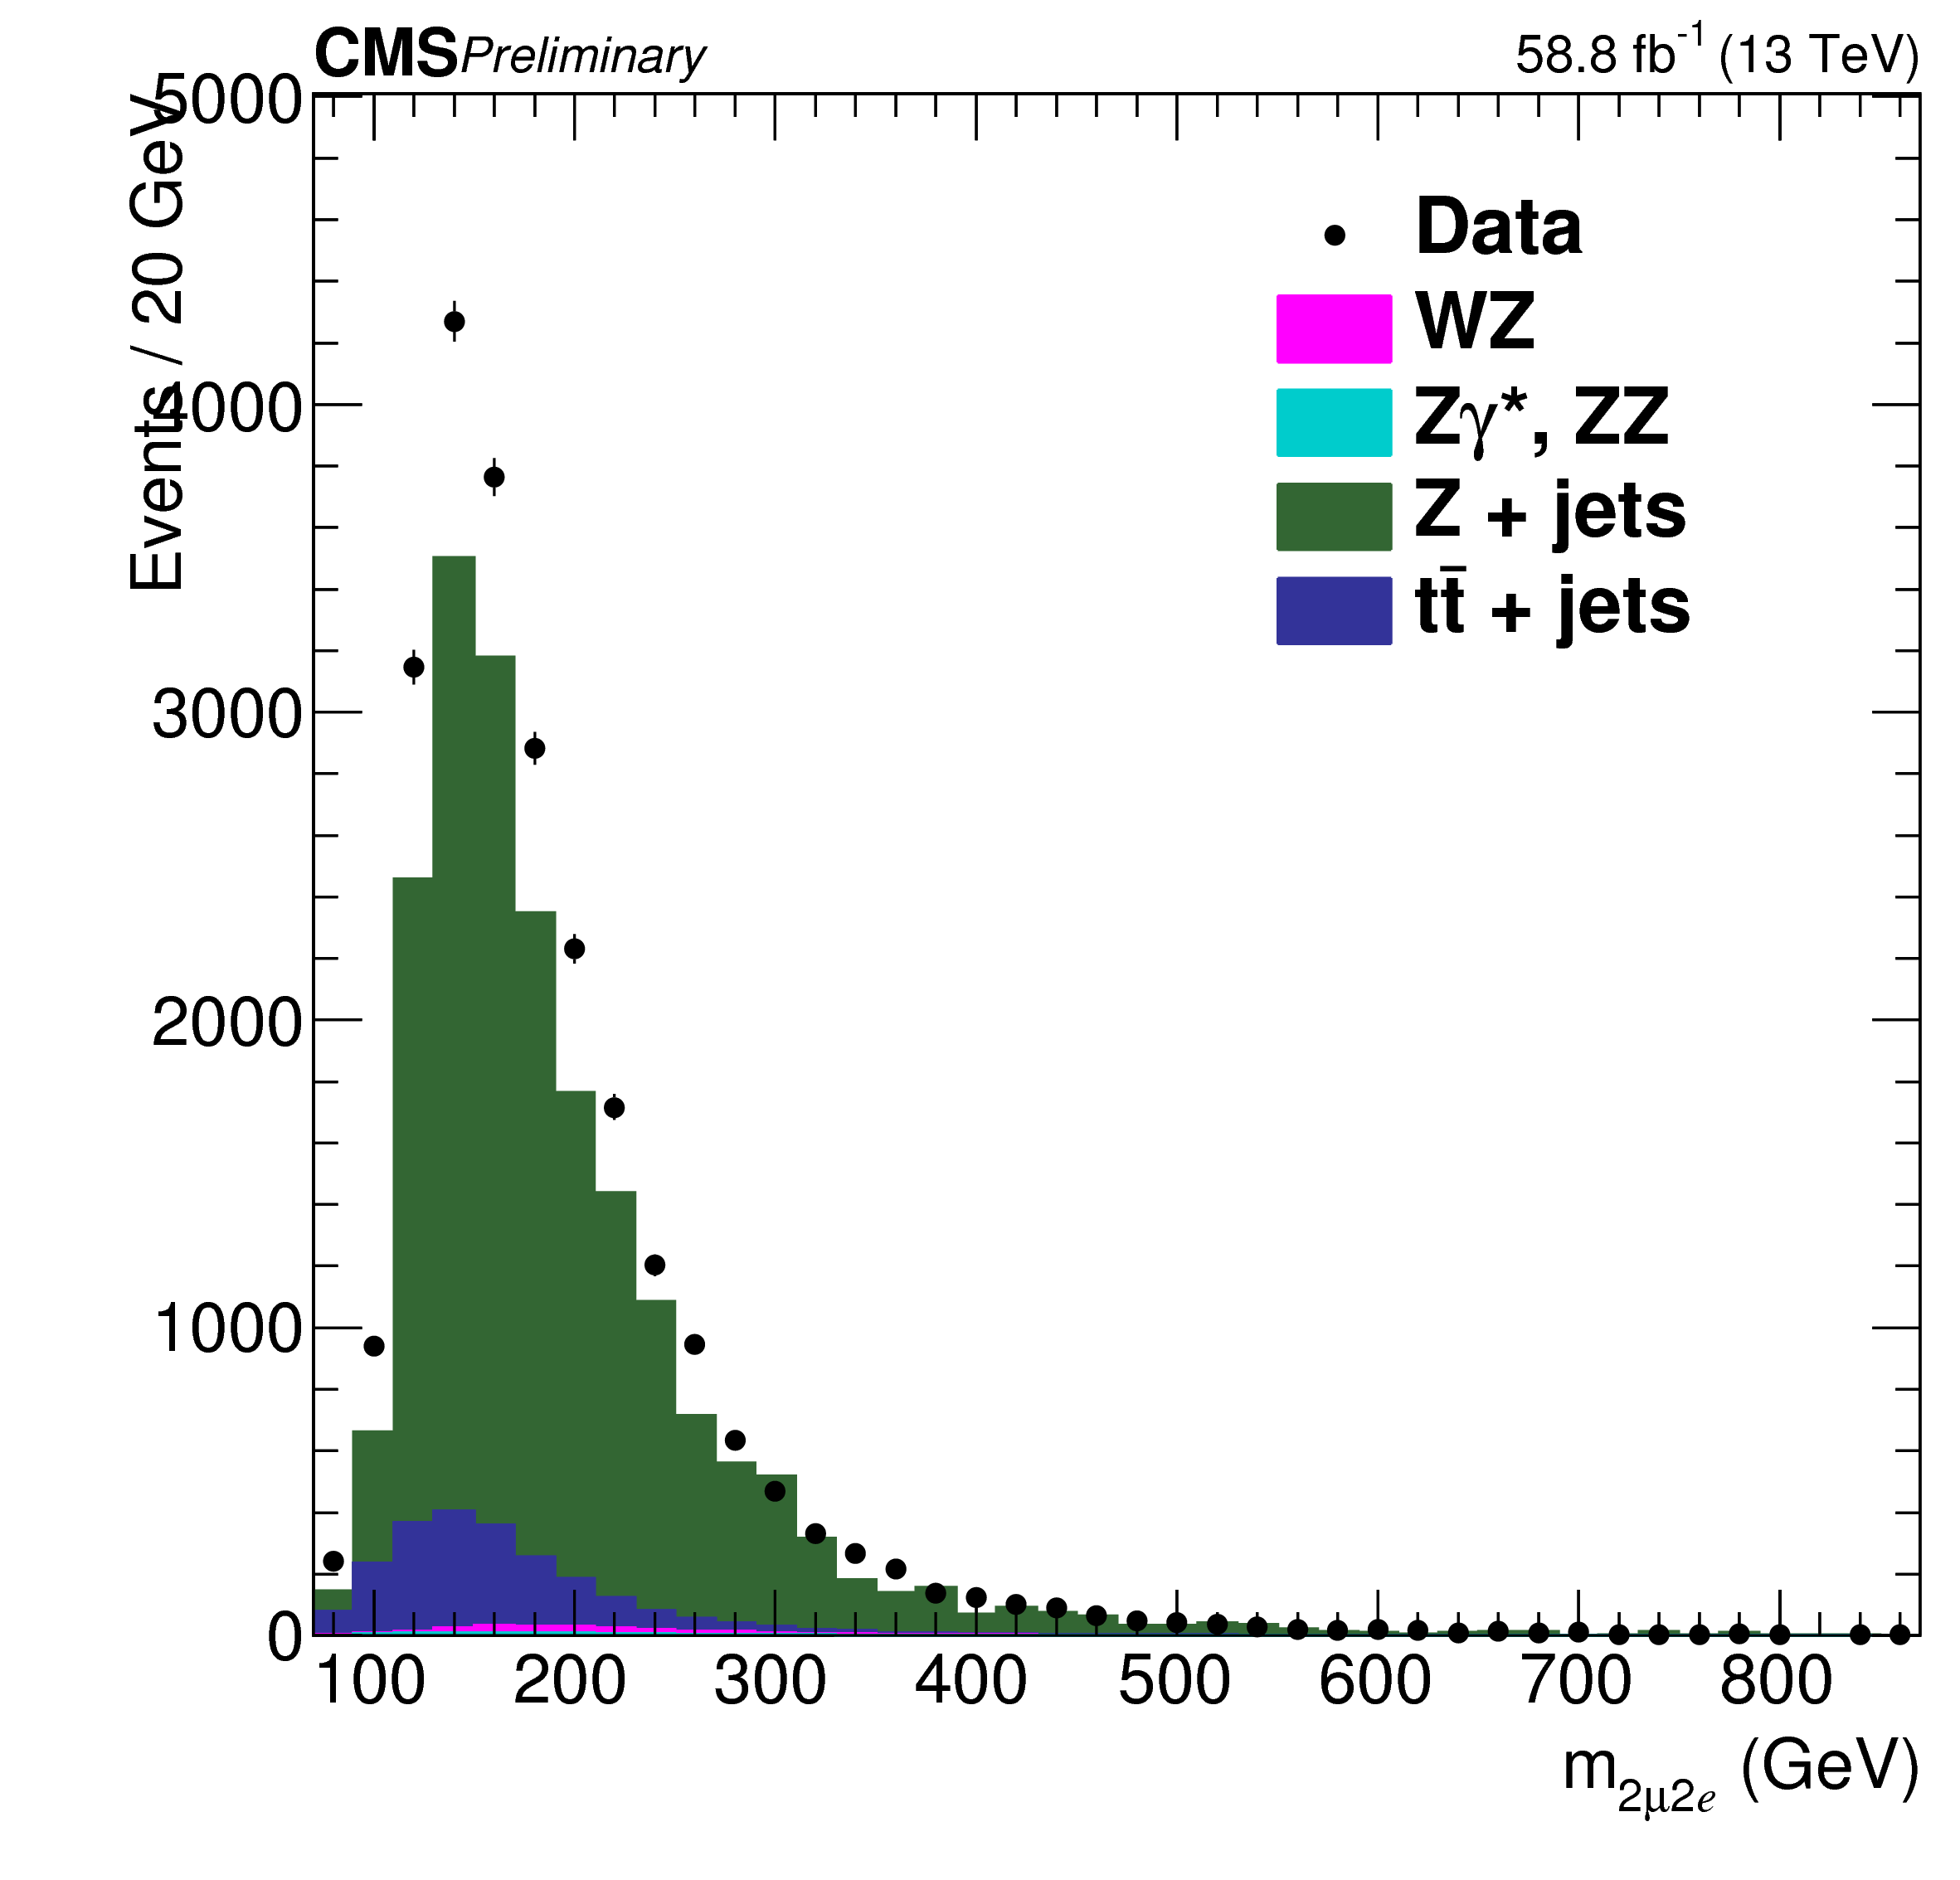
\includegraphics[width=0.45\textwidth]{Figures/RedBkg/M4l_SS_2mu2e_Inclusive.png}}  \\ 
\subfigure[]{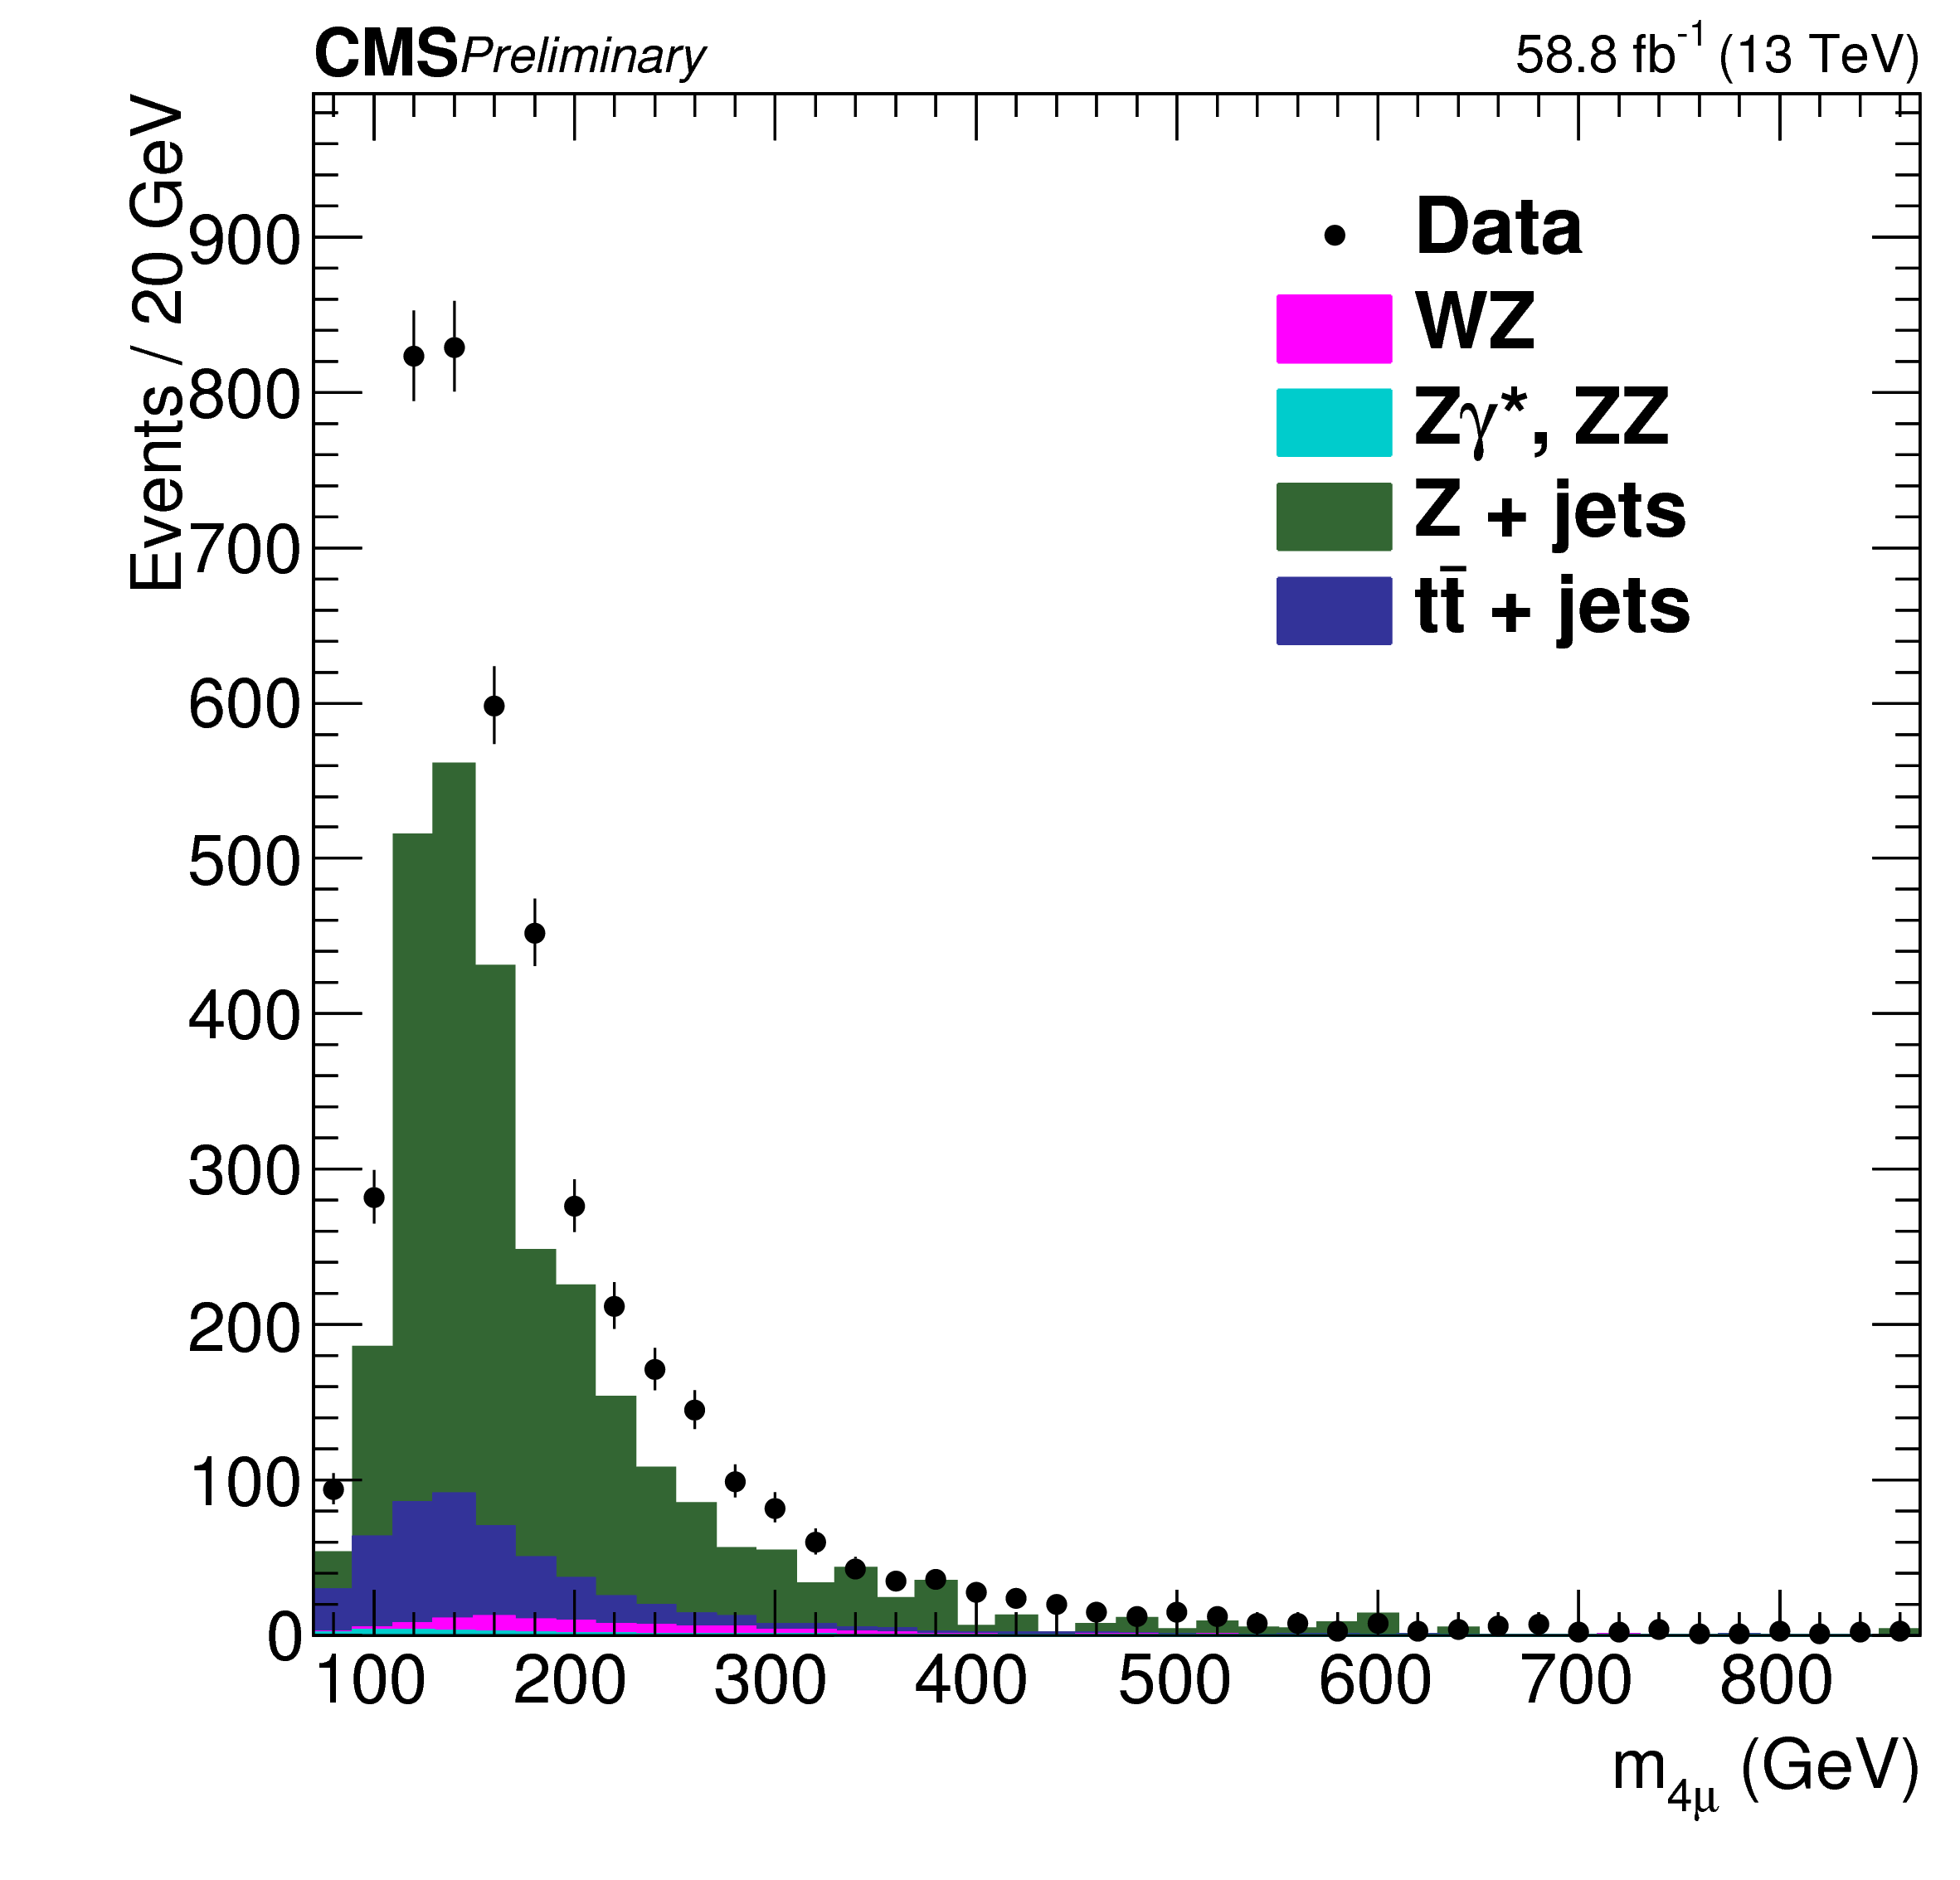
\includegraphics[width=0.45\textwidth]{Figures/RedBkg/M4l_SS_4mu_Inclusive.png}}  
\subfigure[]{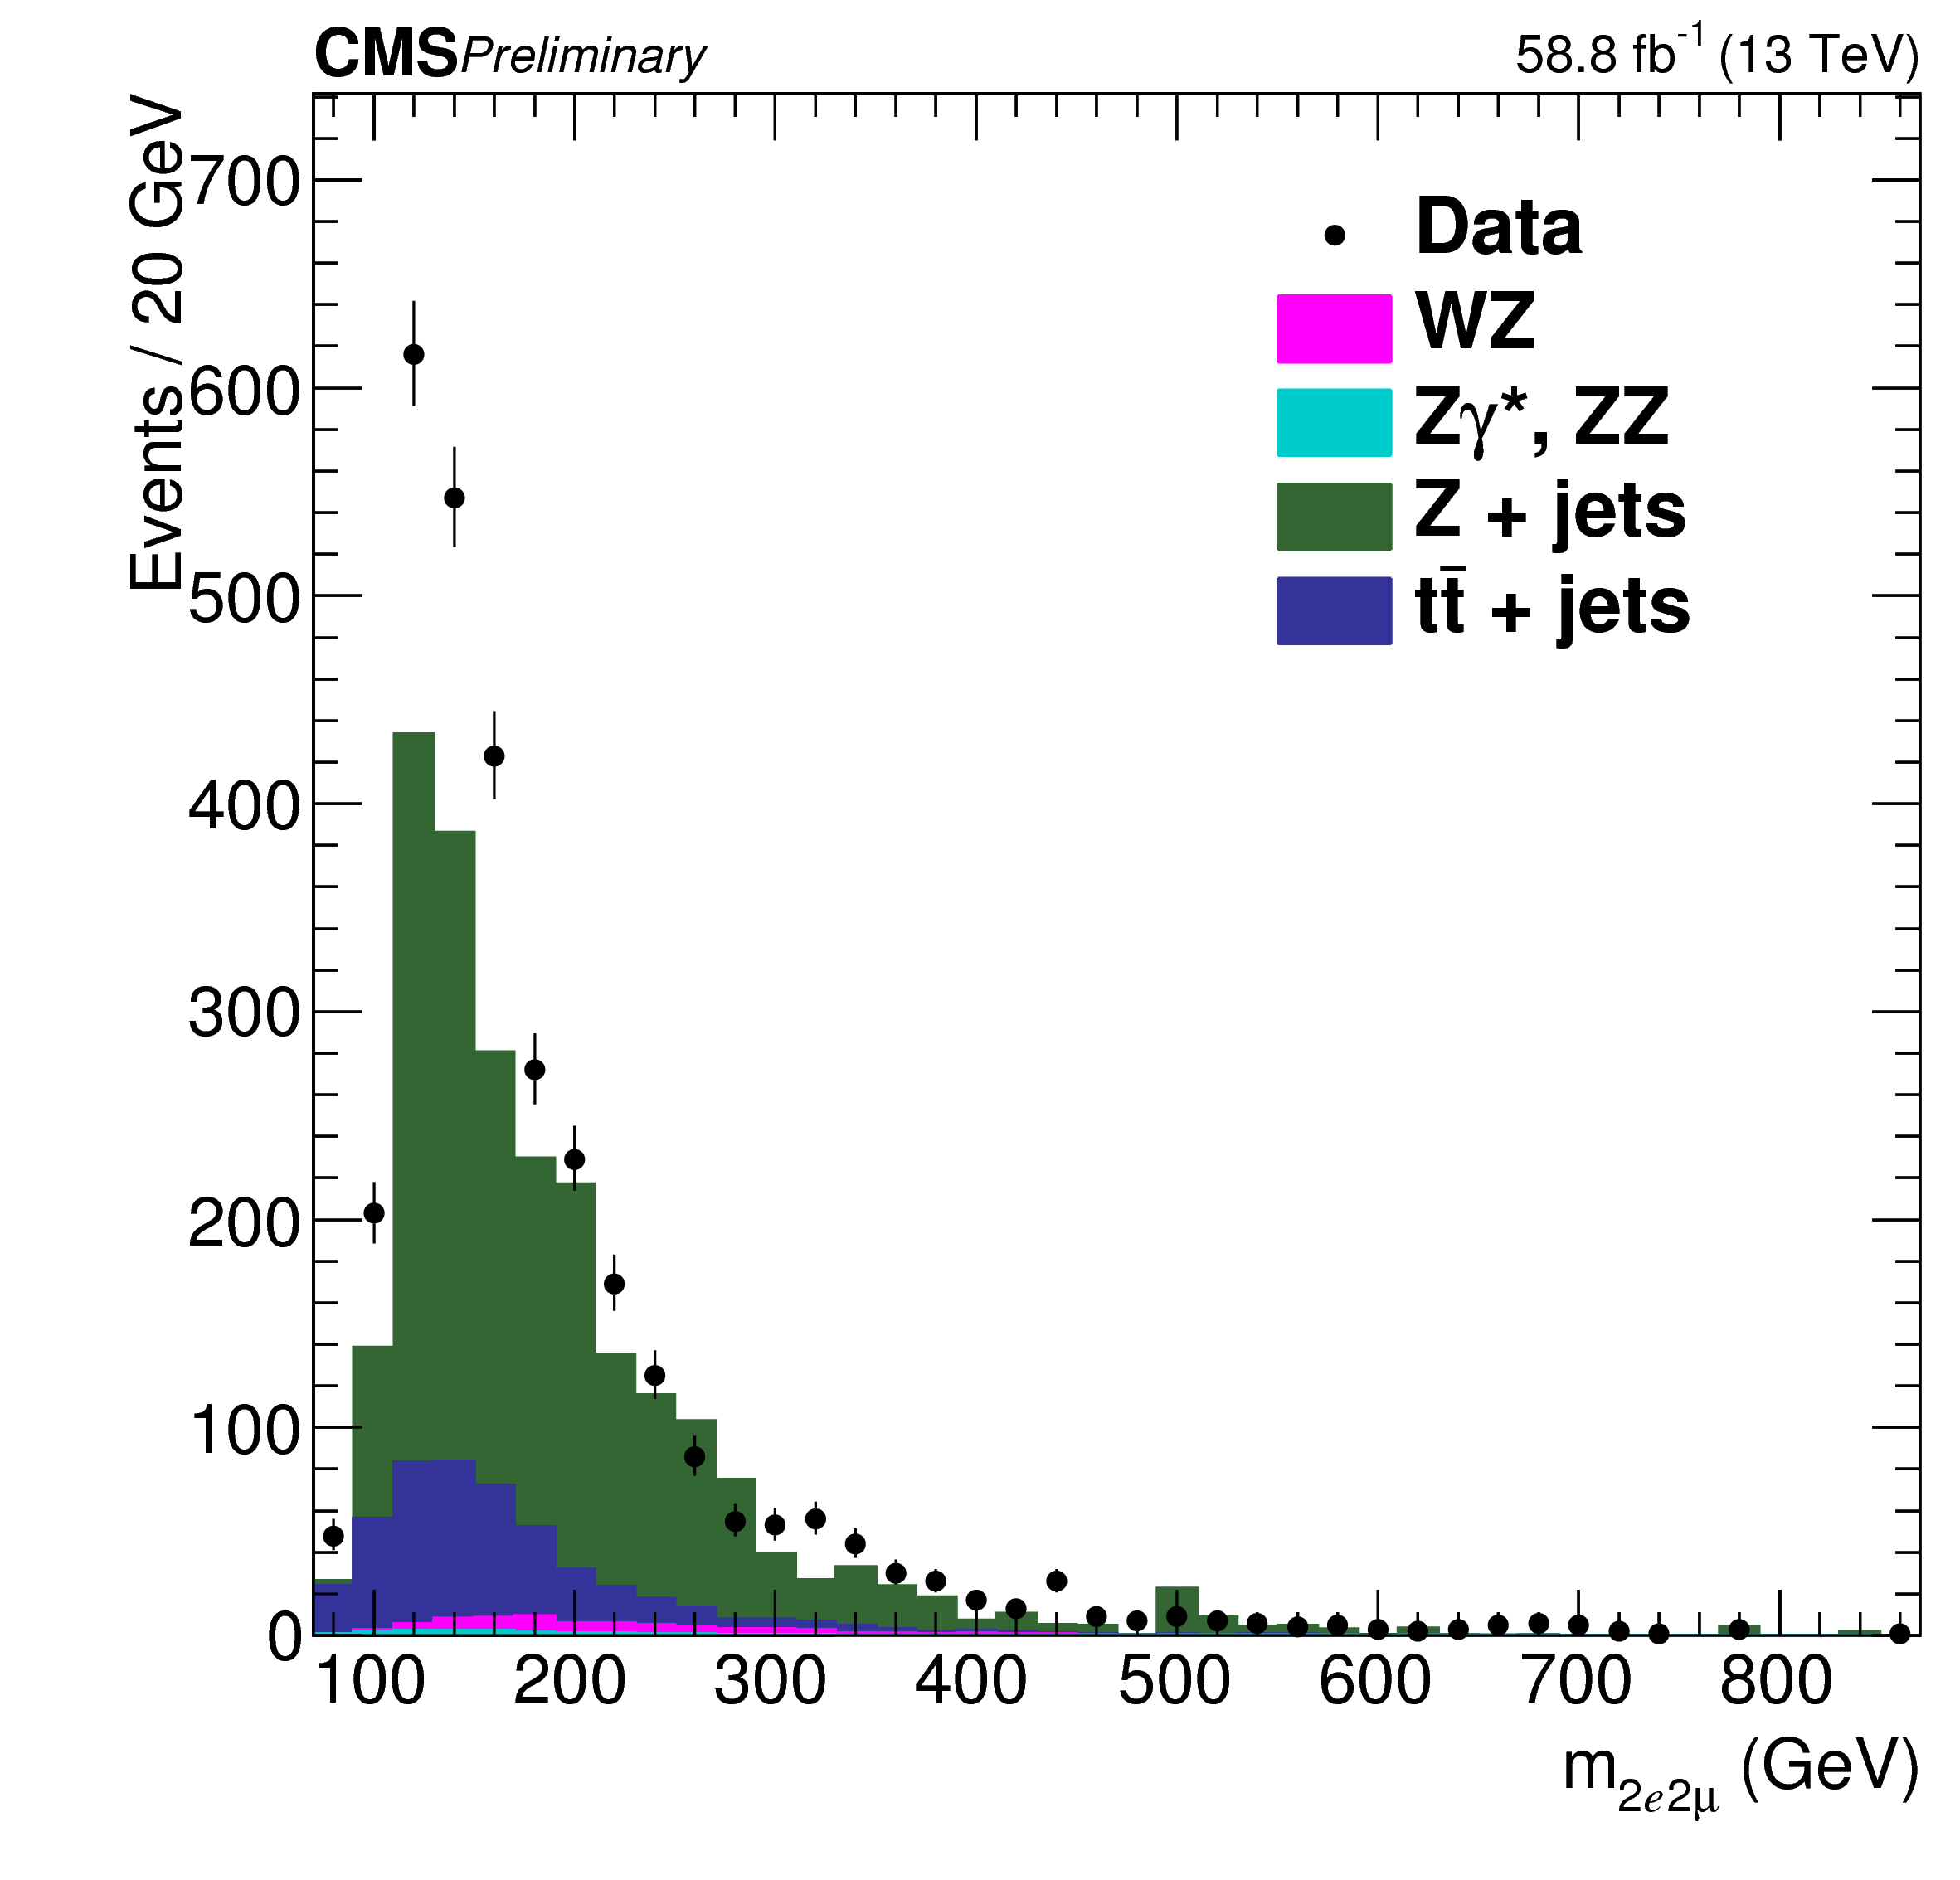
\includegraphics[width=0.45\textwidth]{Figures/RedBkg/M4l_SS_2e2mu_Inclusive.png}} \\ 
\caption{DATA-MC comparison of the SS-SF samples in the Z+X background control samples.
(a) and (b) $4e$ and $2\mu2e$, (c) and (d) $4\mu$ and $2e2\mu$ in 2018 data.  \label{fig:ZjetControlRegionShapes13TeV}}
\end{center}
\end{figure}

The event yields expected from Z+X in the signal region, in the mass range  $m_{4 \ell} > 70~\GeVcc$,  are calculated for each final state and for each of the 22 STXS Stage 1.1. categories defined in Section~\ref{subsec:stxs_cat}. An example for the 4$\Pe$ final state is shown in Table~\ref{tab:ZjetResultsAA_4e}.
The statistical error is due to the event statistics in the control region. 
The systematic is due to error introduced with the missing hits based correction for electrons and the uncertanty in the fake rates in the muon case. 
The background is due to the systematic introduced when estimating the background composition. 
The total error is obtained with a quadrature sum for the statistical, background composition and correction systematics.


\begin{table}[htb!]
\begin{center}
\small
\begin{tabular}{ l | c | c | c | c | c }
\hline
\hline
Category & exp. $N^{\rm Z+X}$ in SR & (stat.) & (syst.) & Total unc.\\
\hline
\hline
ggH\_0J\_PTH\_0\_10           & 0.81 & $\pm 0.22$ & $\pm 0.02 $  & $\pm 0.33 $ \\
\hline
ggH\_0J\_PTH\_10\_200    & 10.8 & $\pm 0.79$ & $\pm 0.20 $  & $\pm 3.33 $ \\
\hline
ggH\_1J\_PTH\_0\_60    & 2.93 & $\pm 0.39$ & $\pm 0.059 $  & $\pm 0.97 $ \\
\hline
ggH\_1J\_PTH\_60\_120    & 2.81 & $\pm 0.38$ & $\pm 0.08 $  & $\pm 0.93 $ \\
\hline
ggH\_2J\_PTH\_0\_60    & 0.89 & $\pm 0.20$ & $\pm 0.02 $  & $\pm 0.33 $ \\
\hline
ggH\_2J\_PTH\_60\_120    & 1.25 & $\pm 0.24$ & $\pm 0.02 $  & $\pm 0.45 $ \\
\hline
ggH\_2J\_PTH\_120\_200    & 0.70 & $\pm 0.18$ & $\pm 0.02 $  & $\pm 0.28 $ \\
\hline
ggH\_PTH\_200    & 0.72 & $\pm 0.16$ & $\pm 0.03 $  & $\pm 0.27 $ \\
\hline
ggH\_VBF    & 0.65 & $\pm 0.16$ & $\pm 0.02 $  & $\pm 0.25 $ \\
\hline
VBF\_1j    & 1.15 & $\pm 0.23$ & $\pm 0.03 $  & $\pm 0.42 $ \\
\hline
VBF\_2j    & 0.34 & $\pm 0.11$ & $\pm 0.01 $  & $\pm 0.15 $ \\
\hline
VBF\_2j\_mjj\_350\_700\_2j    & 0.04 & $\pm 0.04$ & $\pm 0.00 $  & $\pm 0.04 $ \\
\hline
VBF\_2j\_mjj\_GT700\_2j    & 0.06 & $\pm 0.04$ & $\pm 0.00 $  & $\pm 0.04 $ \\
\hline
VBF\_2j\_mjj\_GT350\_3j    & 0.63 & $\pm 0.17$ & $\pm 0.02 $  & $\pm 0.26 $ \\
\hline
VBF\_GT200\_2J    & 0.06 & $\pm 0.03$ & $\pm 0.00 $  & $\pm 0.04 $ \\
\hline
VH\_Had    & 1.10 & $\pm 0.21$ & $\pm 0.03 $  & $\pm 0.39 $ \\
\hline
VBF\_rest\_VH    & 0.15 & $\pm 0.06$ & $\pm 0.01 $  & $\pm 0.08 $ \\
\hline
VH\_lep\_0\_150    & 0.69 & $\pm 0.18$ & $\pm 0.02 $  & $\pm 0.27 $ \\
\hline
VH\_Lep\_GT150    & 0.11 & $\pm 0.06$ & $\pm 0.00 $  & $\pm 0.07 $ \\
\hline
ttH\_Lep    & 0.32 & $\pm 0.11$ & $\pm 0.01 $  & $\pm 0.14 $ \\
\hline
ttH\_Had    & 0.51 & $\pm 0.13$ & $\pm 0.01 $  & $\pm 0.20 $ \\
\hline

\hline
\hline
Inclusive          & 24.92 & $\pm 1.18$ & $\pm 0.42 $  & $\pm 7.58 $ \\
\hline
\hline
\end{tabular}
\end{center}
\caption{Number of $4\Pe$ events in the SS-SF control region for $\usedLumiC$ of 2018 data, and expected number of Z+X$\to4\Pe$ events in the signal region as predicted from the SS method. Systematical error shown listed in table is only due to fake rate variation. Background composition component of 30\% is taken into account in the total uncertainty.
\label{tab:ZjetResultsAA_4e}}
\end{table}


